% classnames = {'wave2','balance','bend','box','clap','dance','wave1'};
\begin{figure}
	\centering 
	\begin{subfigure}[b]{1\linewidth}
		\centering
		\begin{tabular}{c|cccc}
			\raisebox{1cm}{\textbf{Input}} &
			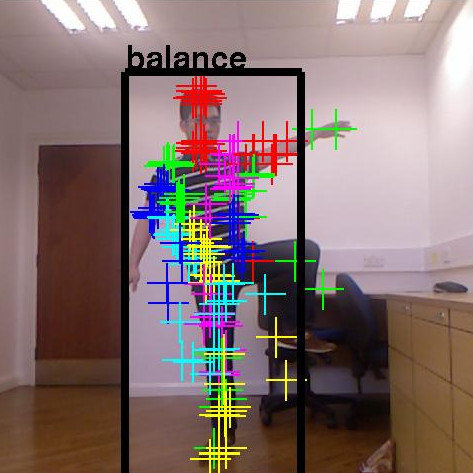
\includegraphics[height=2.3cm]{fig/body/APE/balc1.jpg} & 
			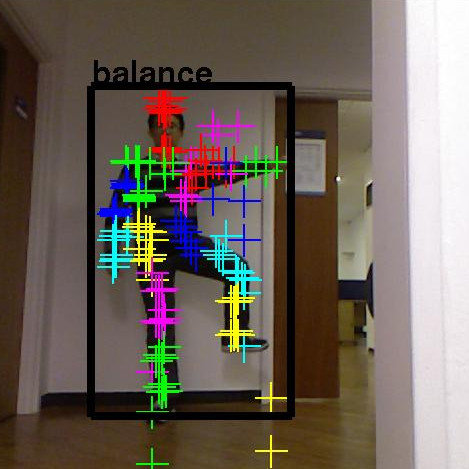
\includegraphics[height=2.3cm]{fig/body/APE/balc2.jpg} &
			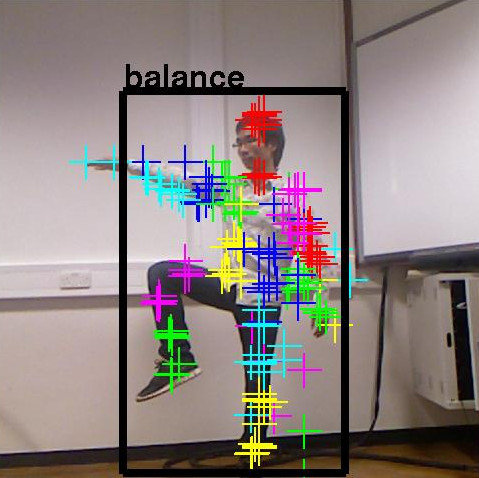
\includegraphics[height=2.3cm]{fig/body/APE/balc3.jpg} & 
			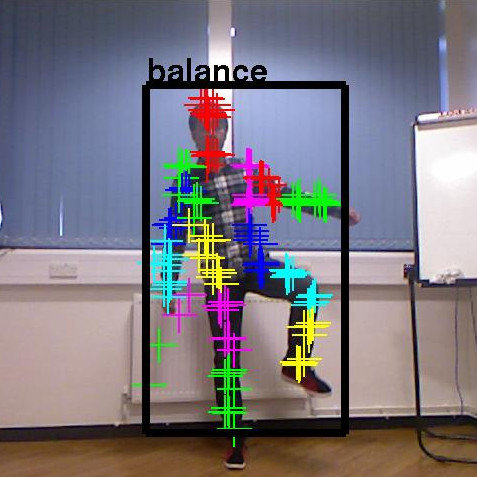
\includegraphics[height=2.3cm]{fig/body/APE/balc4.jpg} \\
			\raisebox{1cm}{\textbf{3D pose}} &
			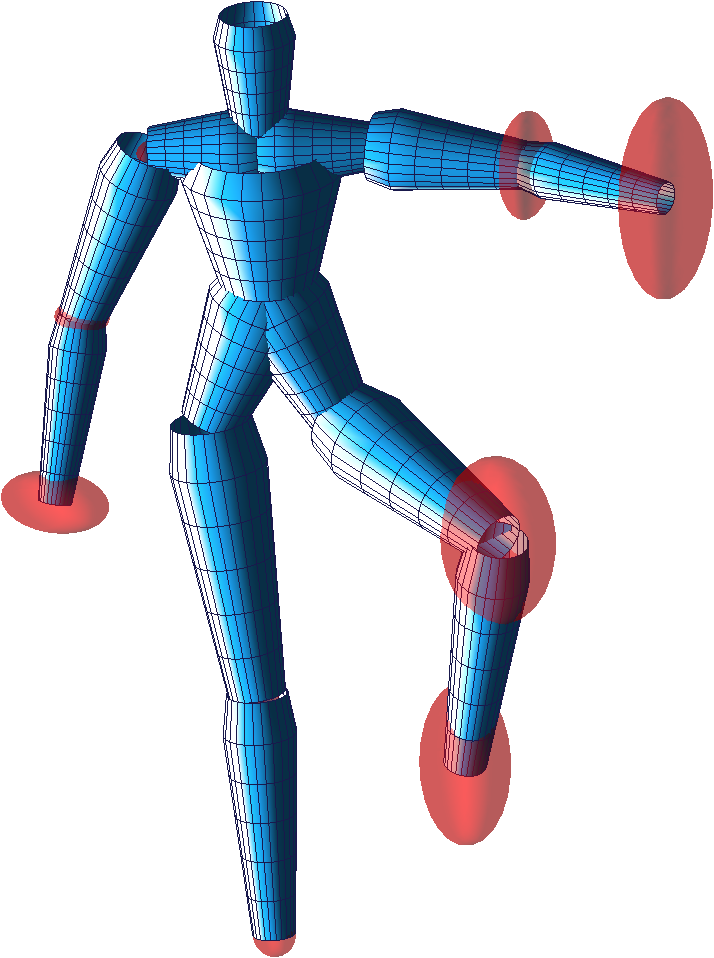
\includegraphics[height=2.3cm]{fig/body/APE/balc1.png} & 
			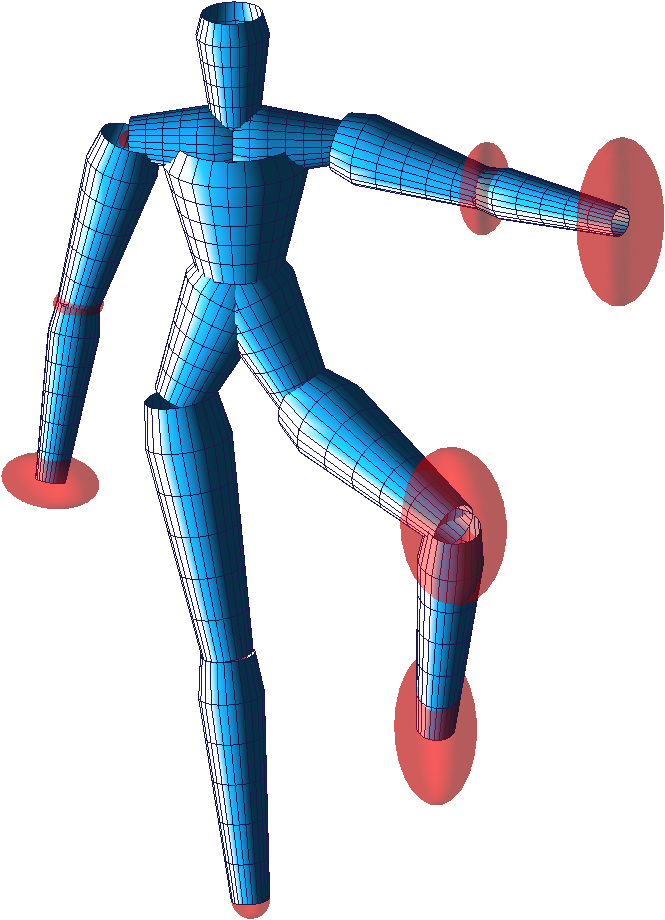
\includegraphics[height=2.3cm]{fig/body/APE/balc2.png} &
			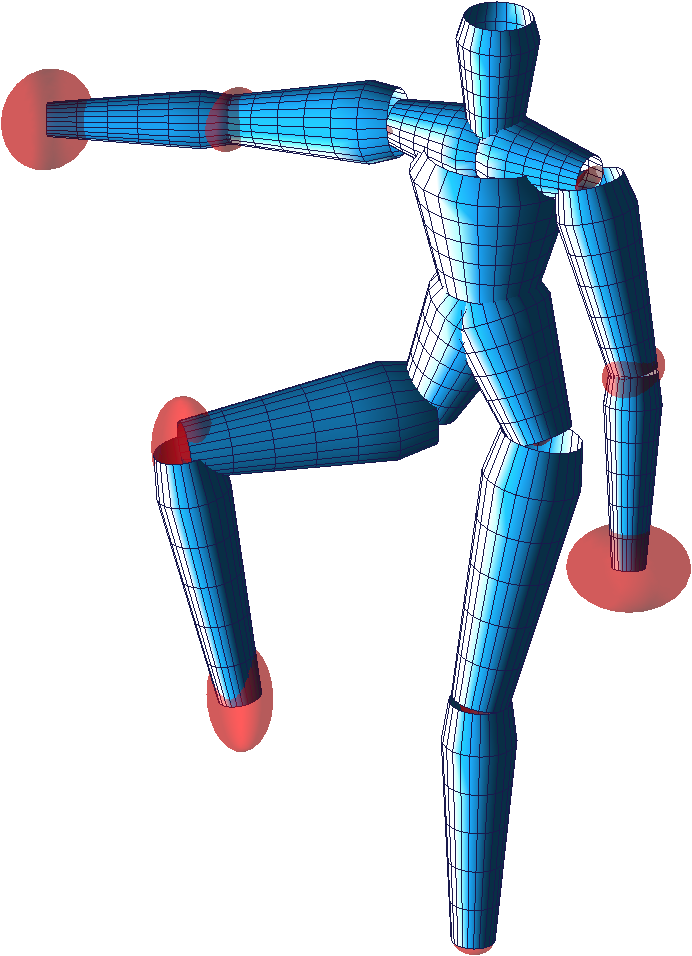
\includegraphics[height=2.3cm]{fig/body/APE/balc3.png} & 
			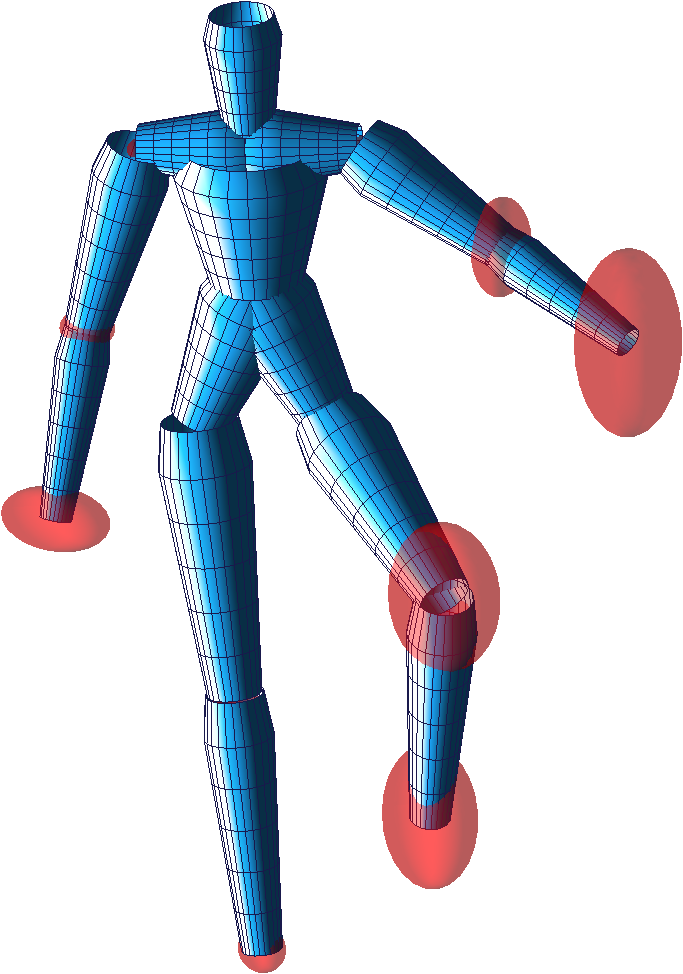
\includegraphics[height=2.3cm]{fig/body/APE/balc4.png} 
		\end{tabular}
		\subcaption{Balance}
		\label{fig/body/APE/balc} 
	\end{subfigure}
	\begin{subfigure}[b]{1\linewidth}
		\centering
		\begin{tabular}{c|cccc}
			\raisebox{1cm}{\textbf{Input}} &
			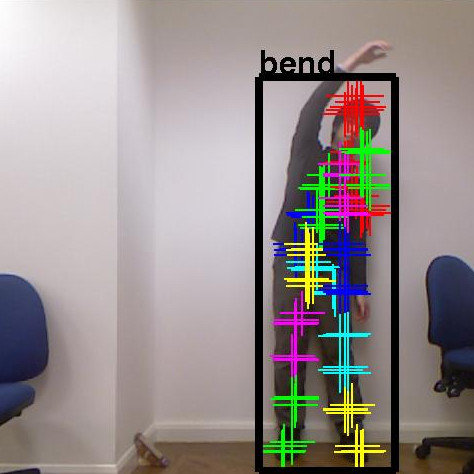
\includegraphics[height=2.3cm]{fig/body/APE/bend1.jpg} & 
			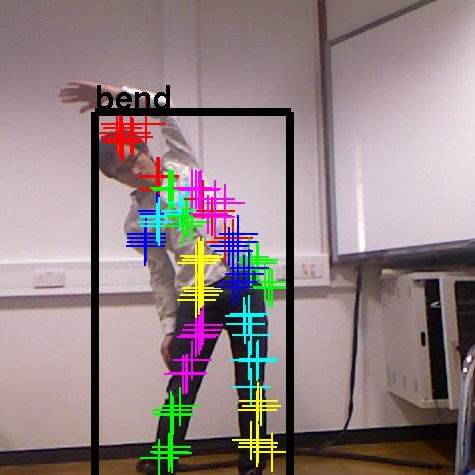
\includegraphics[height=2.3cm]{fig/body/APE/bend2.jpg} &
			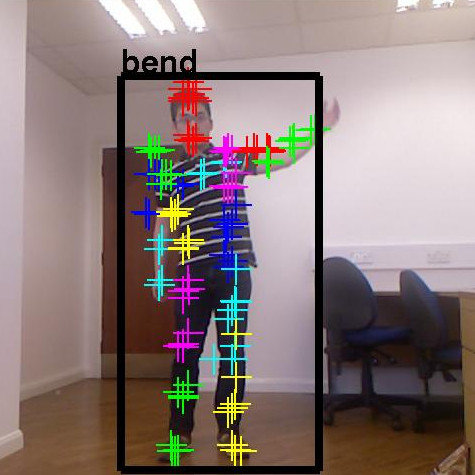
\includegraphics[height=2.3cm]{fig/body/APE/bend3.jpg} & 
			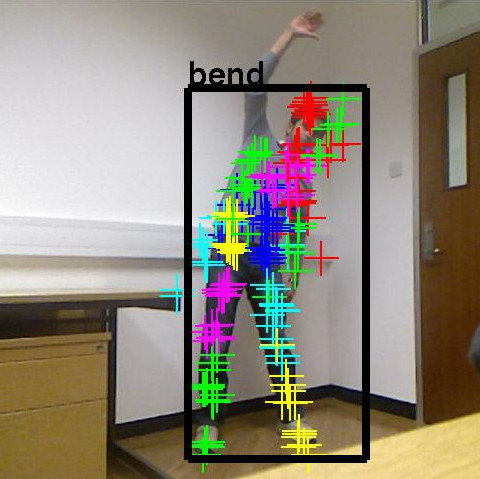
\includegraphics[height=2.3cm]{fig/body/APE/bend4.jpg} \\
			\raisebox{1cm}{\textbf{3D pose}} &
			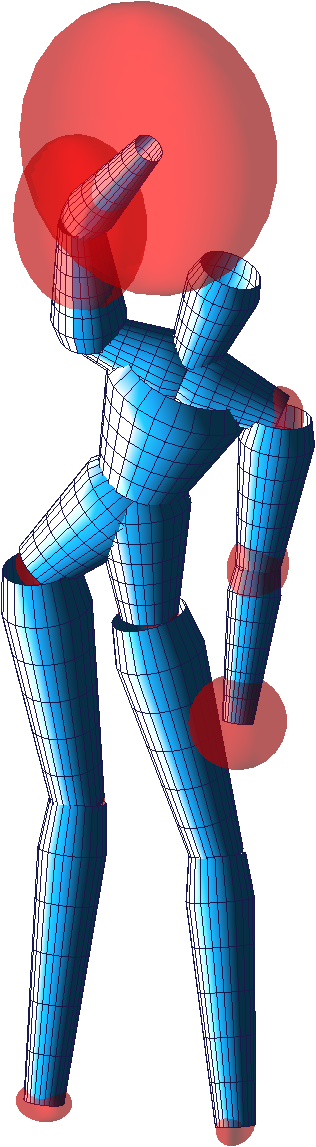
\includegraphics[height=2.3cm]{fig/body/APE/bend1.png} & 
			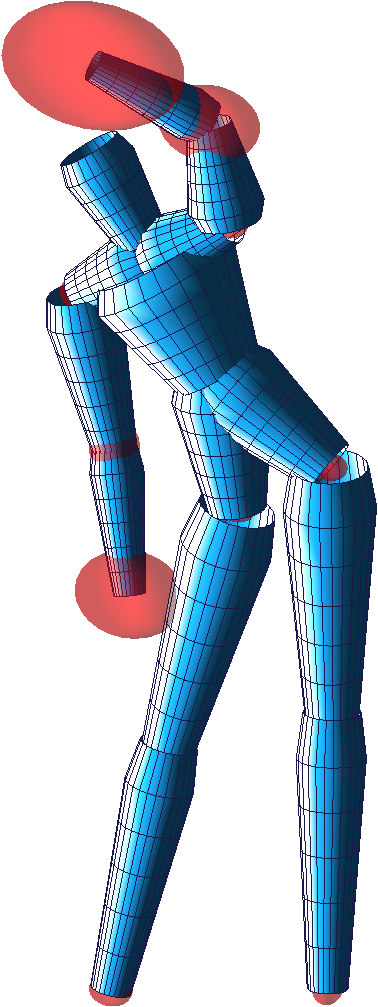
\includegraphics[height=2.3cm]{fig/body/APE/bend2.png} &
			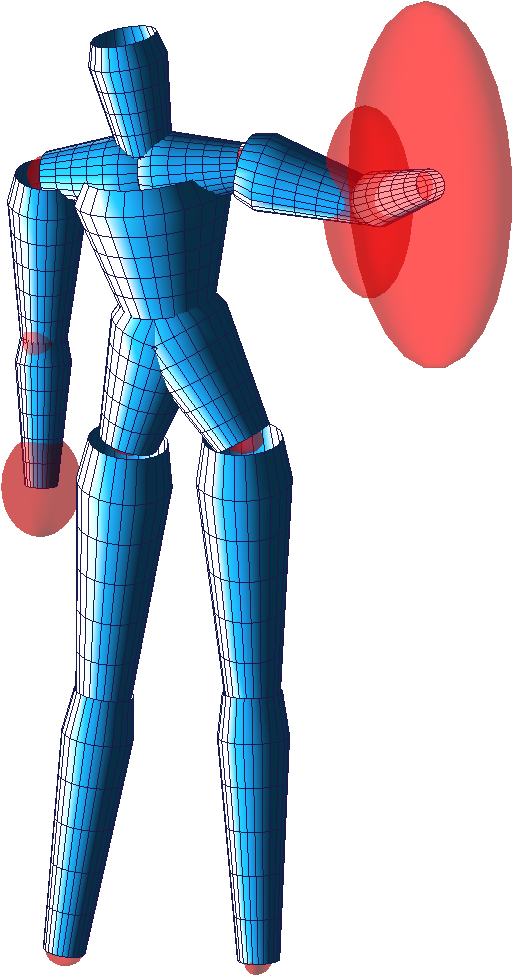
\includegraphics[height=2.3cm]{fig/body/APE/bend3.png} & 
			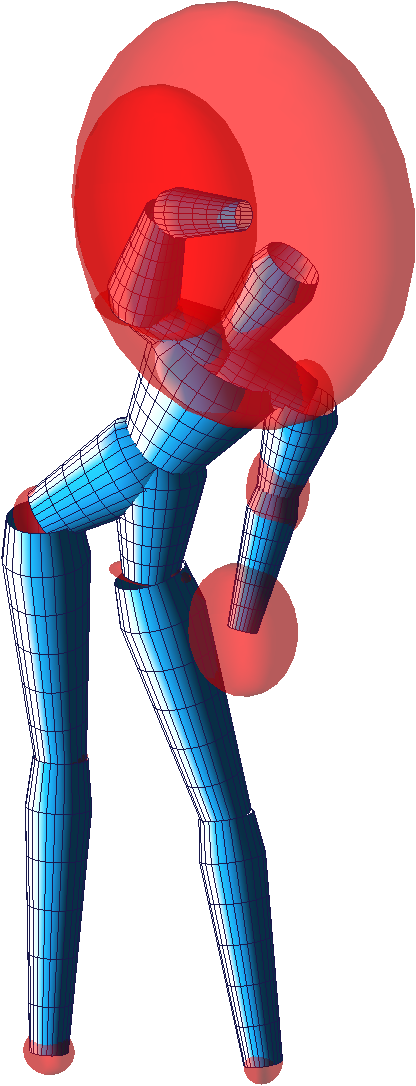
\includegraphics[height=2.3cm]{fig/body/APE/bend4.png} 
		\end{tabular}
		\subcaption{Bend}
		\label{fig/body/APE/bend} 
	\end{subfigure}
	\begin{subfigure}[b]{1\linewidth}
		\centering
		\begin{tabular}{c|cccc}
			\raisebox{1cm}{\textbf{Input}} &
			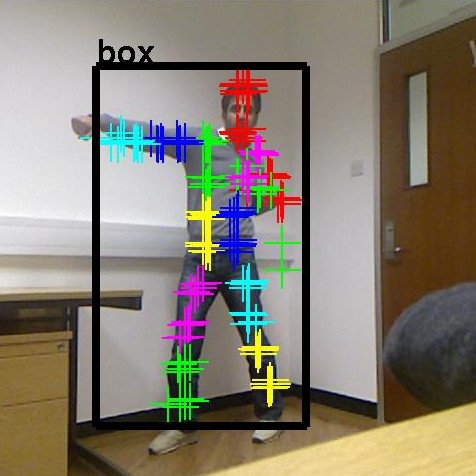
\includegraphics[height=2.3cm]{fig/body/APE/boxx1.jpg} & 
			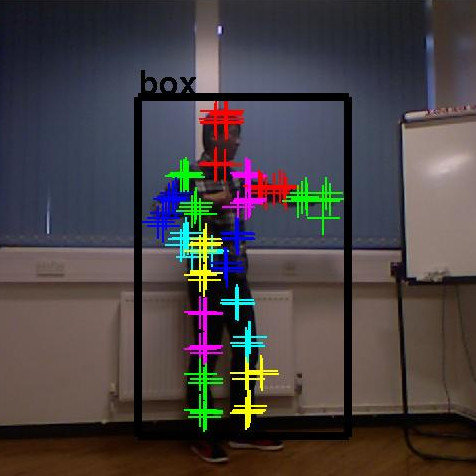
\includegraphics[height=2.3cm]{fig/body/APE/boxx2.jpg} &
			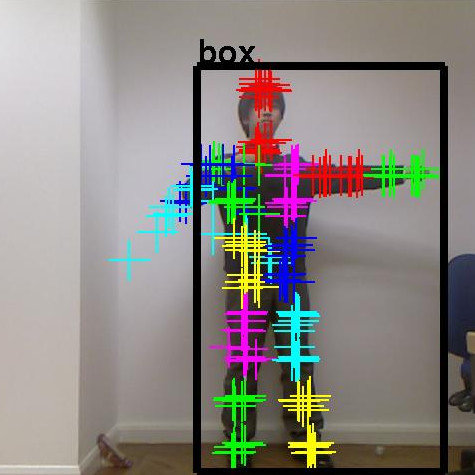
\includegraphics[height=2.3cm]{fig/body/APE/boxx3.jpg} & 
			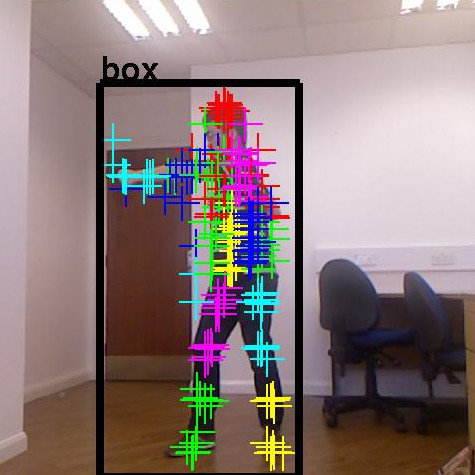
\includegraphics[height=2.3cm]{fig/body/APE/boxx4.jpg} \\
			\raisebox{1cm}{\textbf{3D pose}} &
			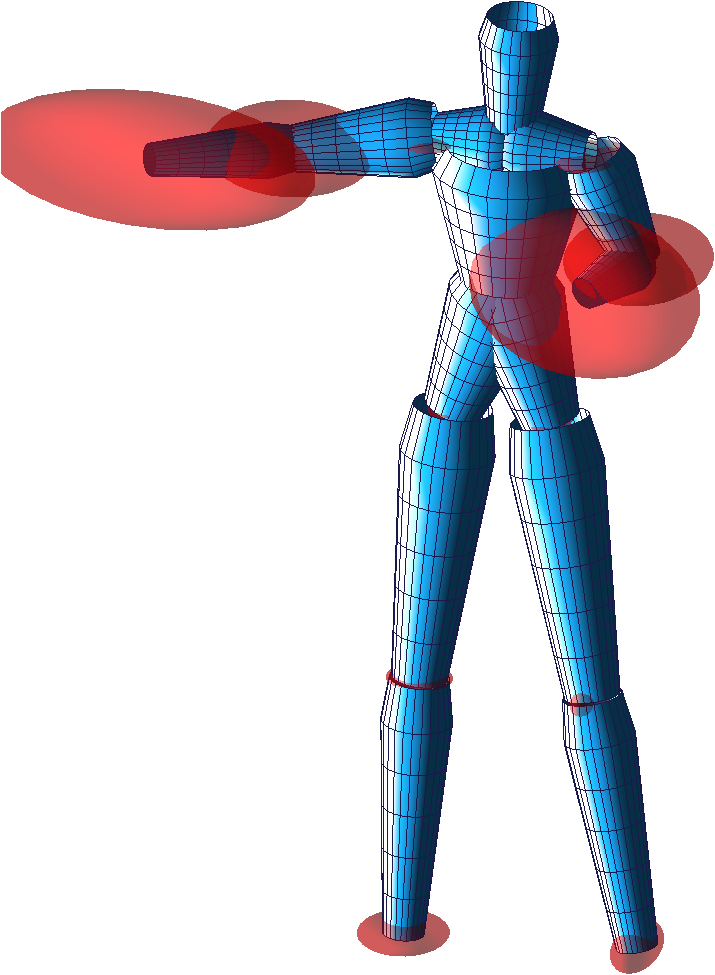
\includegraphics[height=2.3cm]{fig/body/APE/boxx1.png} & 
			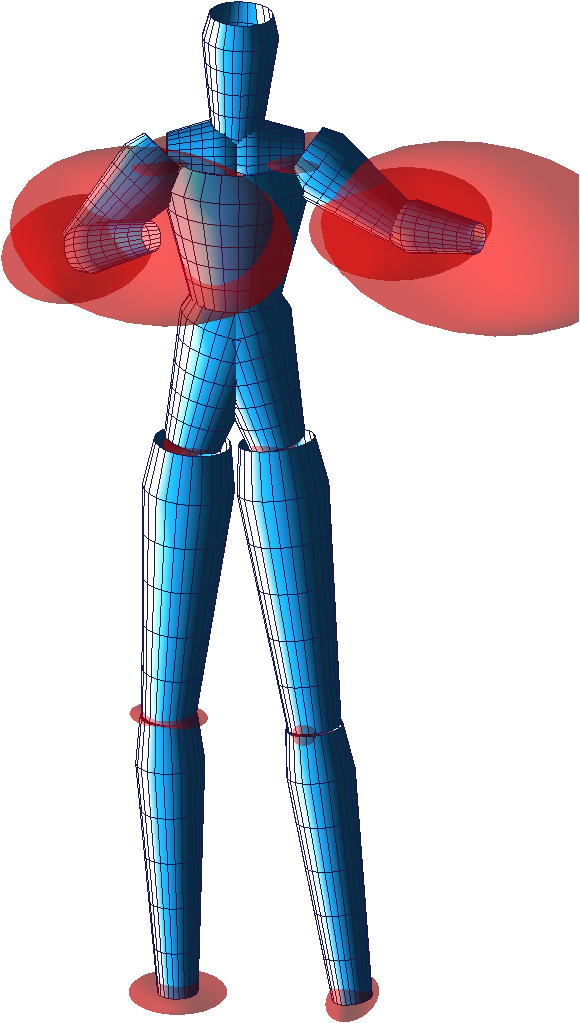
\includegraphics[height=2.3cm]{fig/body/APE/boxx2.png} &
			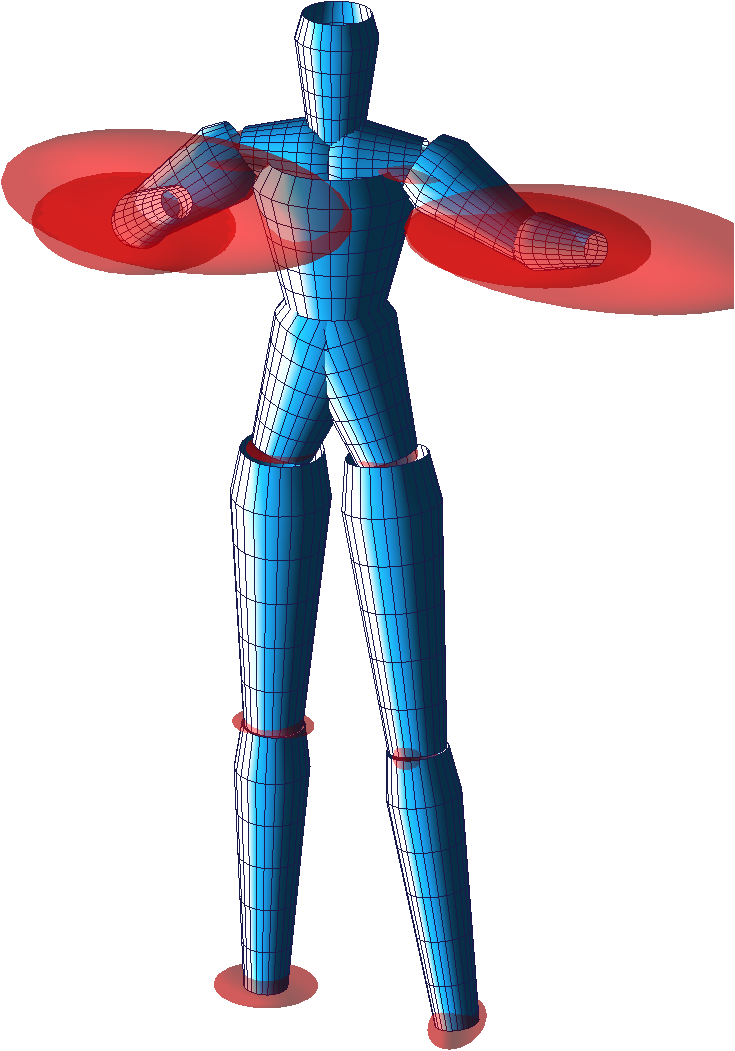
\includegraphics[height=2.3cm]{fig/body/APE/boxx3.png} & 
			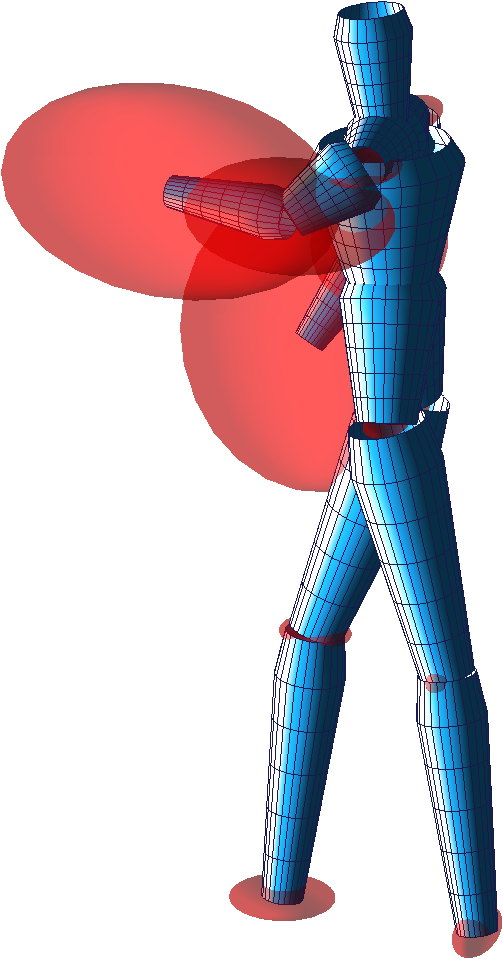
\includegraphics[height=2.3cm]{fig/body/APE/boxx4.png} 
		\end{tabular}
		\subcaption{Box}
		\label{fig/body/APE/boxx} 
	\end{subfigure}
	\caption{\textbf{3-D pose estimation results of APE dataset.} From top to bottom: (a) balance, (b) bend, and (c) box.}
	\label{fig/body/APE1}
\end{figure}

\begin{figure}
	\centering 
	\begin{subfigure}[b]{1\linewidth}
		\centering
		\begin{tabular}{c|cccc}
			\raisebox{1cm}{\textbf{Input}} &
			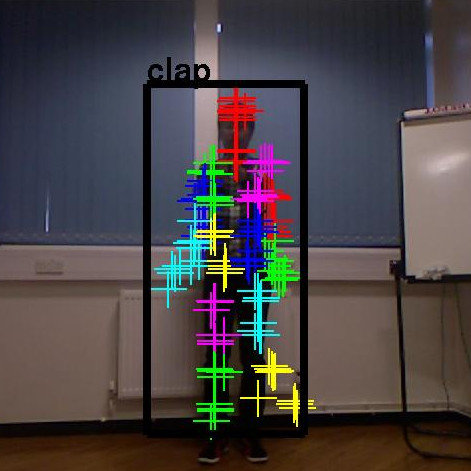
\includegraphics[height=2.3cm]{fig/body/APE/clap1.jpg} & 
			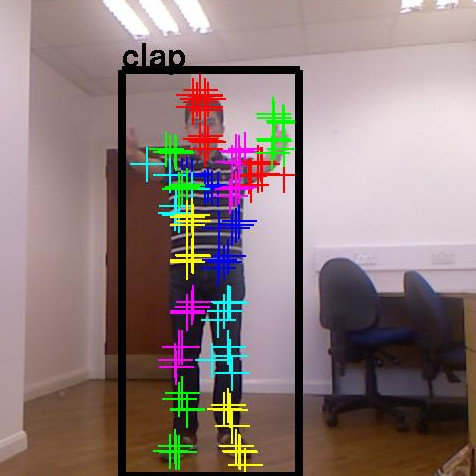
\includegraphics[height=2.3cm]{fig/body/APE/clap2.jpg} &
			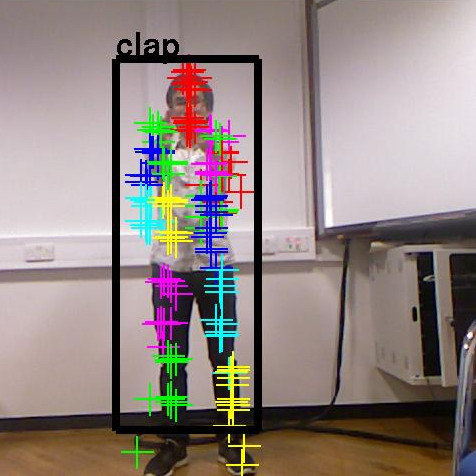
\includegraphics[height=2.3cm]{fig/body/APE/clap3.jpg} & 
			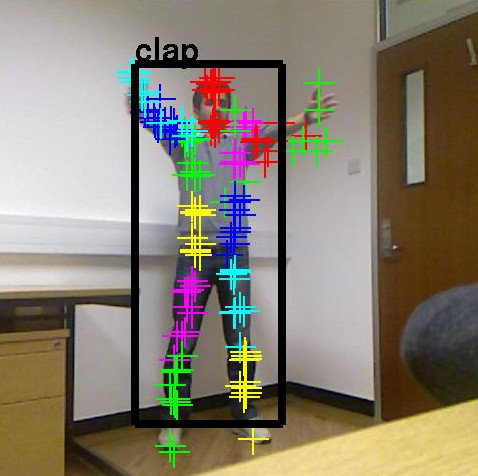
\includegraphics[height=2.3cm]{fig/body/APE/clap4.jpg} \\
			\raisebox{1cm}{\textbf{3D pose}} &
			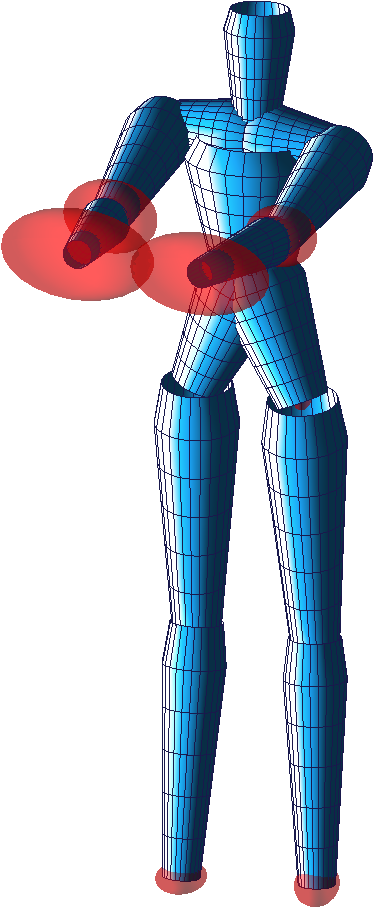
\includegraphics[height=2.3cm]{fig/body/APE/clap1.png} & 
			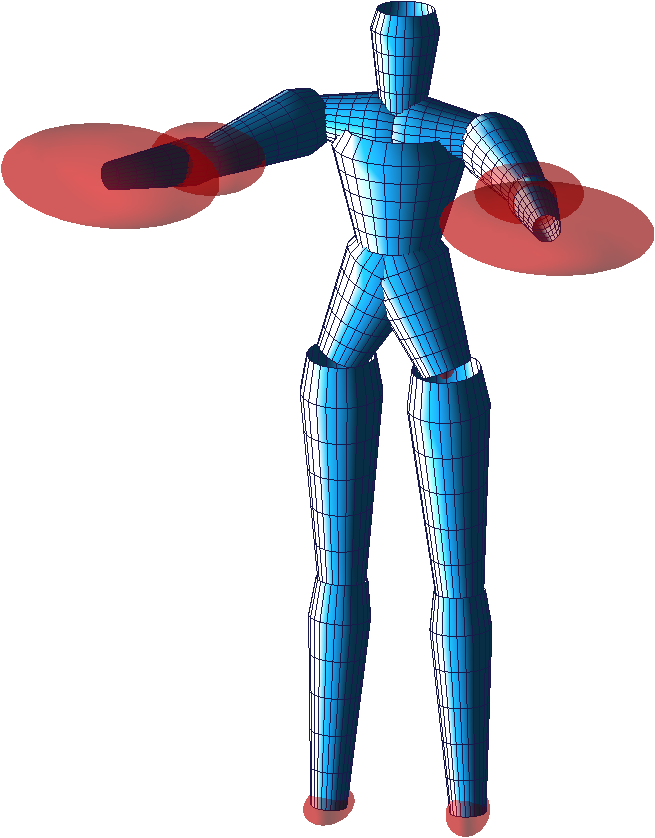
\includegraphics[height=2.3cm]{fig/body/APE/clap2.png} &
			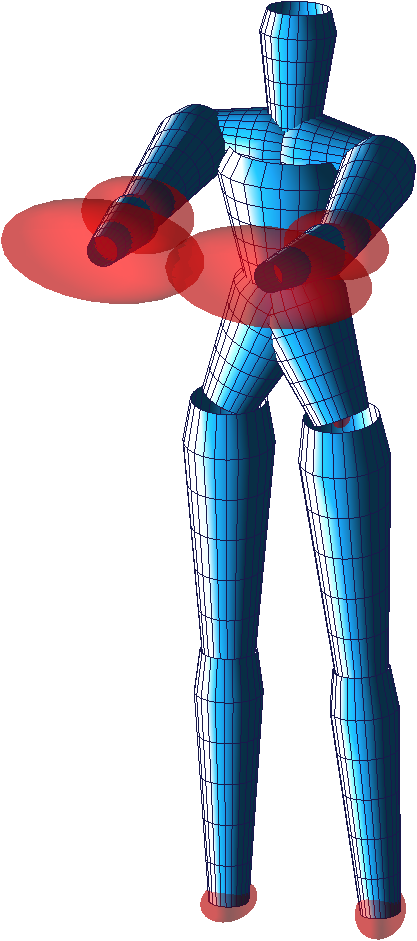
\includegraphics[height=2.3cm]{fig/body/APE/clap3.png} & 
			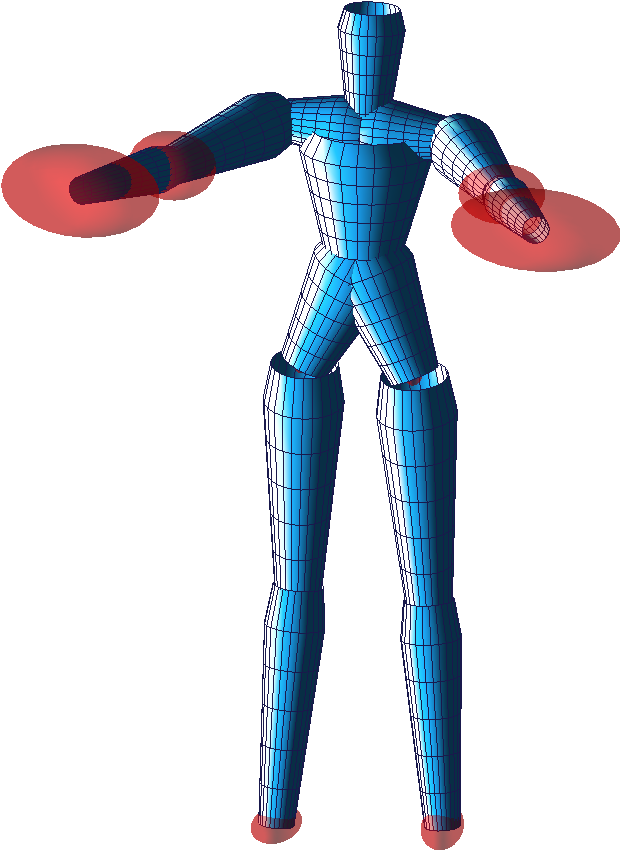
\includegraphics[height=2.3cm]{fig/body/APE/clap4.png} 
		\end{tabular}
		\subcaption{Clap}
		\label{fig/body/APE/clap} 
	\end{subfigure}
	\begin{subfigure}[b]{1\linewidth}
		\centering
		\begin{tabular}{c|cccc}
			\raisebox{1cm}{\textbf{Input}} &
			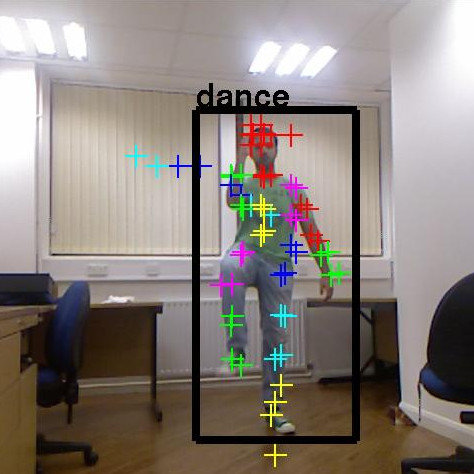
\includegraphics[height=2.3cm]{fig/body/APE/dance1.jpg} & 
			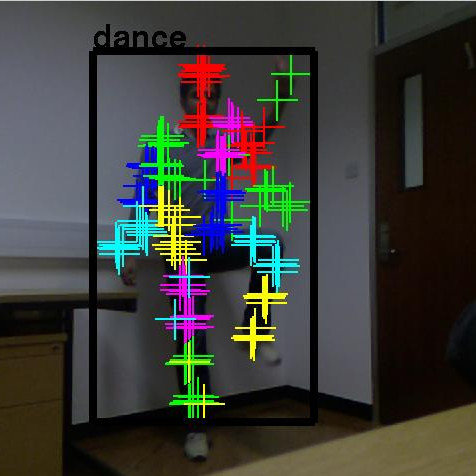
\includegraphics[height=2.3cm]{fig/body/APE/dance2.jpg} &
			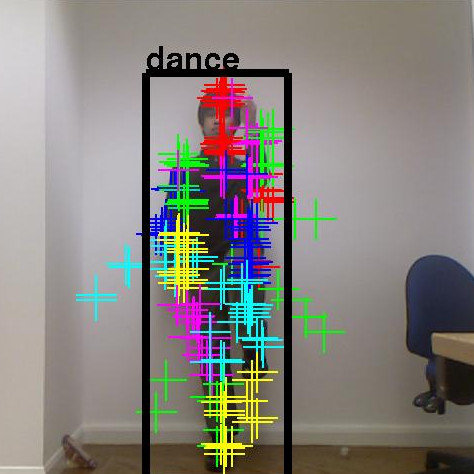
\includegraphics[height=2.3cm]{fig/body/APE/dance3.jpg} & 
			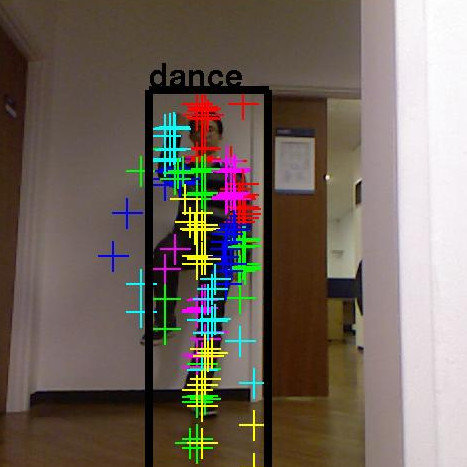
\includegraphics[height=2.3cm]{fig/body/APE/dance4.jpg} \\
			\raisebox{1cm}{\textbf{3D pose}} &
			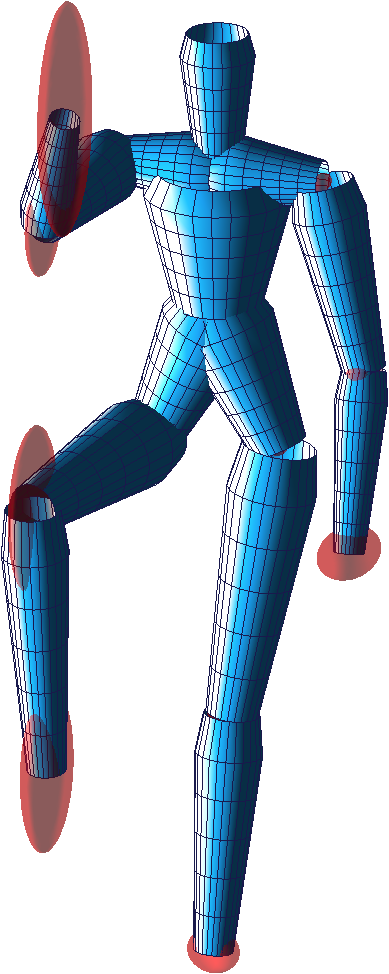
\includegraphics[height=2.3cm]{fig/body/APE/dance1.png} & 
			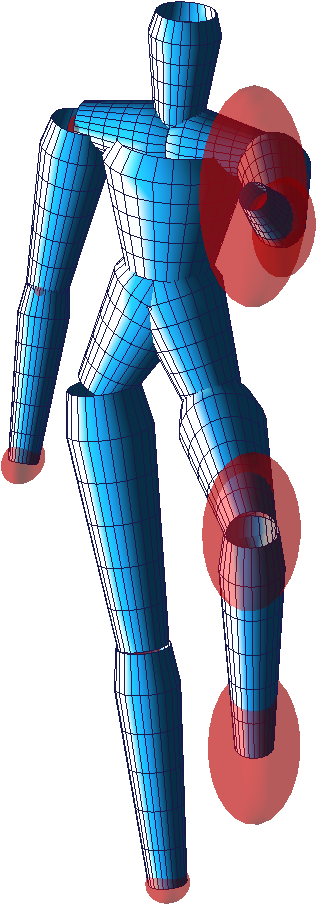
\includegraphics[height=2.3cm]{fig/body/APE/dance2.png} &
			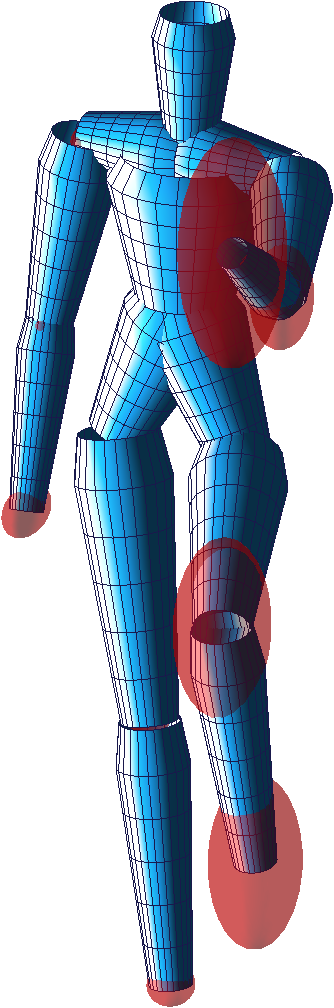
\includegraphics[height=2.3cm]{fig/body/APE/dance3.png} & 
			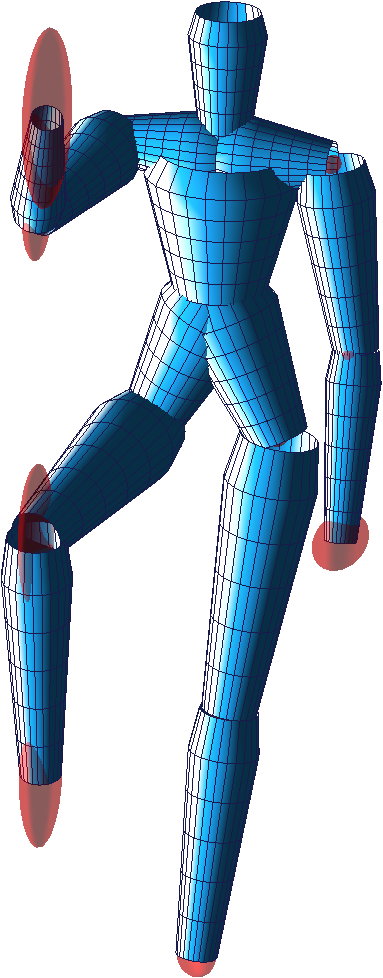
\includegraphics[height=2.3cm]{fig/body/APE/dance4.png} 
		\end{tabular}
		\subcaption{Dance}
		\label{fig/body/APE/dance} 
	\end{subfigure}
	\begin{subfigure}[b]{1\linewidth}
		\centering
		\begin{tabular}{c|cccc}
			\raisebox{1cm}{\textbf{Input}} &
			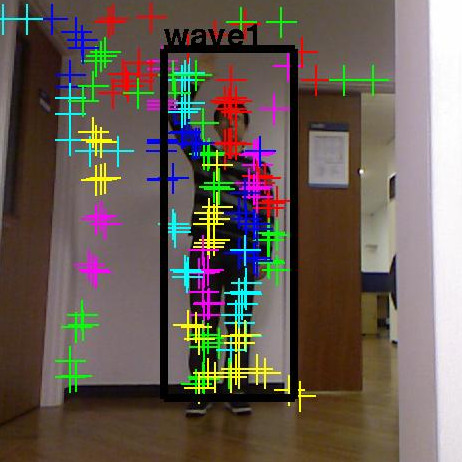
\includegraphics[height=2.3cm]{fig/body/APE/wave11.jpg} & 
			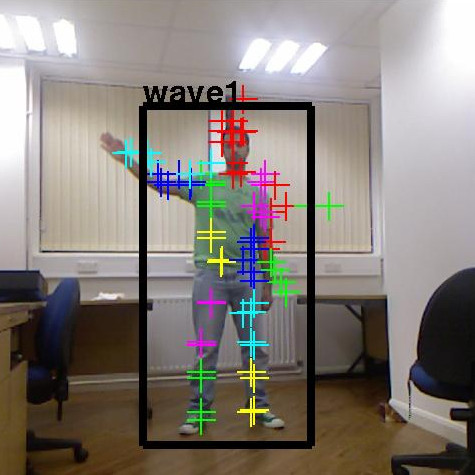
\includegraphics[height=2.3cm]{fig/body/APE/wave12.jpg} &
			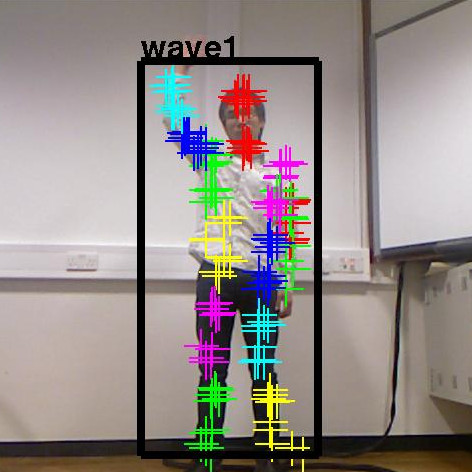
\includegraphics[height=2.3cm]{fig/body/APE/wave13.jpg} & 
			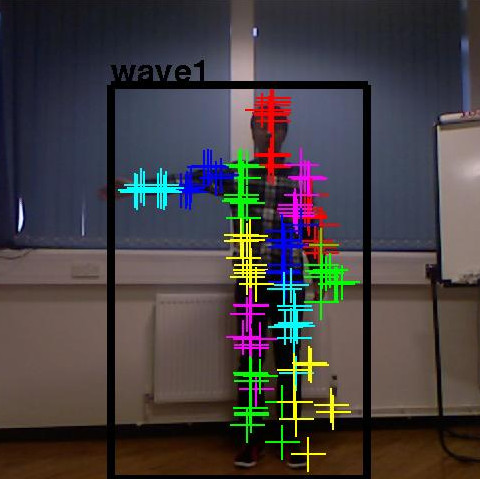
\includegraphics[height=2.3cm]{fig/body/APE/wave14.jpg} \\
			\raisebox{1cm}{\textbf{3D pose}} &
			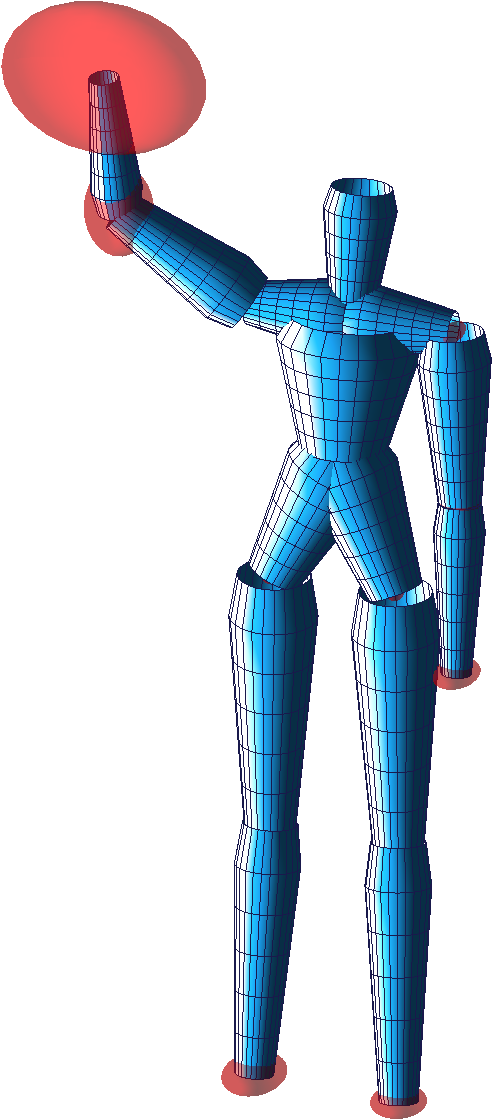
\includegraphics[height=2.3cm]{fig/body/APE/wave11.png} & 
			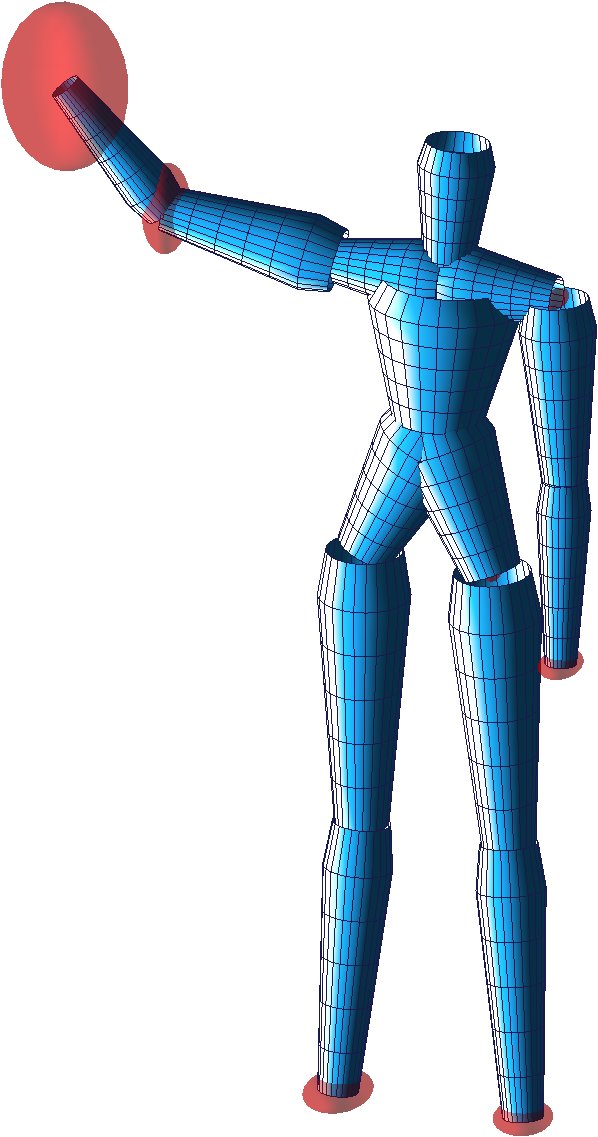
\includegraphics[height=2.3cm]{fig/body/APE/wave12.png} &
			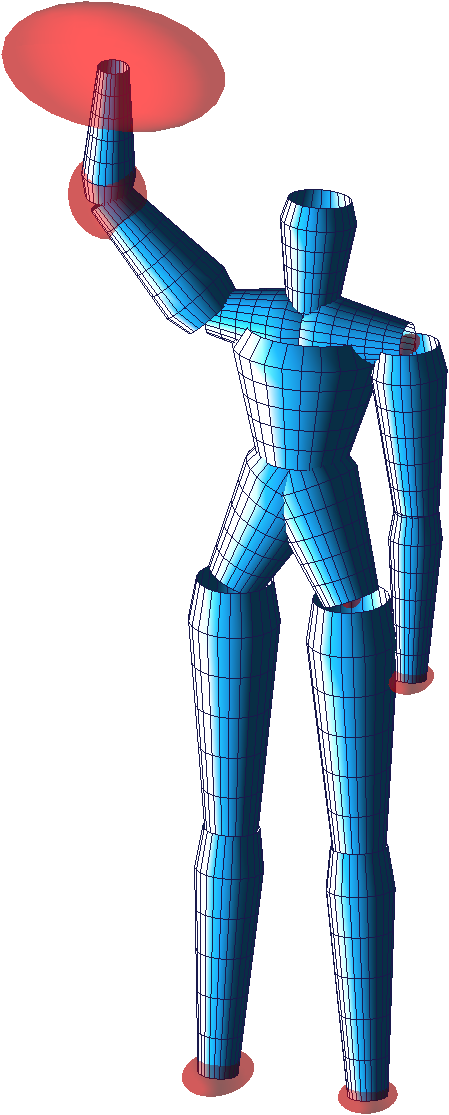
\includegraphics[height=2.3cm]{fig/body/APE/wave13.png} & 
			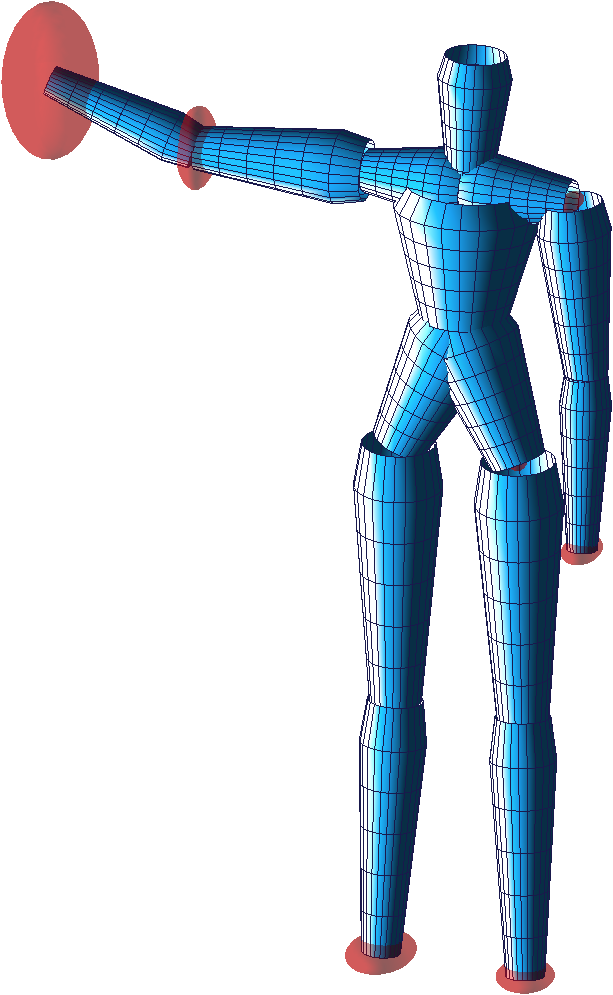
\includegraphics[height=2.3cm]{fig/body/APE/wave14.png} 
		\end{tabular}
		\subcaption{Wave 1}
		\label{fig/body/APE/wave1} 
	\end{subfigure}
	\caption{\textbf{3-D pose estimation results of APE dataset.} From top to bottom: (a) clap, (b) dance, and (c) wave 1}
	\label{fig/body/APE2}
\end{figure}

\begin{figure}
	\centering 
	\begin{tabular}{c|cccc}
		\raisebox{1cm}{\textbf{Input}} &
		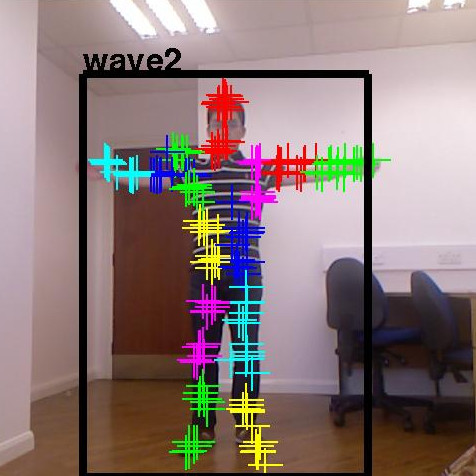
\includegraphics[height=2.3cm]{fig/body/APE/wave21.jpg} & 
		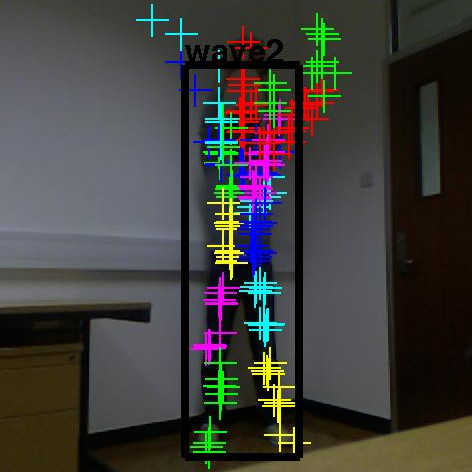
\includegraphics[height=2.3cm]{fig/body/APE/wave22.jpg} &
		\includegraphics[height=2.3cm]{fig/body/APE/wave23.jpg} & 
		\includegraphics[height=2.3cm]{fig/body/APE/wave24.jpg} \\
		\raisebox{1cm}{\textbf{3D pose}} &
		\includegraphics[height=2.3cm]{fig/body/APE/wave21.png} & 
		\includegraphics[height=2.3cm]{fig/body/APE/wave22.png} &
		\includegraphics[height=2.3cm]{fig/body/APE/wave23.png} & 
		\includegraphics[height=2.3cm]{fig/body/APE/wave24.png} 
	\end{tabular}
	\label{fig/body/APE/wave2} 
	\caption{\textbf{3-D pose estimation results of the ``wave 2'' action class.}}
	\label{fig/body/APE3}
\end{figure}

\begin{figure}
	\centering 
	\begin{tabular}{c}
		\raisebox{-0.3cm}{\textbf{Input}} \\ 
		\raisebox{-2.1cm}{\textbf{3D pose}}
	\end{tabular} 
	\begin{tabular}{c|}
		\vbox to 4.6cm {\vfil
			\hbox to 1mm{}%
			\vfil
		}
	\end{tabular}
	\begin{subfigure}[t]{0.18\linewidth} \centering
		\includegraphics[height=2.3cm]{fig/body/APE/benderr.jpg} \\
		\includegraphics[height=2.3cm]{fig/body/APE/benderr.png} 
		\subcaption{Bend}
		\label{fig/body/APEerr1}
	\end{subfigure}
	\begin{subfigure}[t]{0.18\linewidth} \centering
		\includegraphics[height=2.3cm]{fig/body/APE/boxxerr.jpg} \\
		\includegraphics[height=2.3cm]{fig/body/APE/boxxerr.png} 
		\subcaption{Box}
		\label{fig/body/APEerr2}
	\end{subfigure}
	\begin{subfigure}[t]{0.18\linewidth} \centering
		\includegraphics[height=2.3cm]{fig/body/APE/boxerr2.jpg} \\
		\includegraphics[height=2.3cm]{fig/body/APE/boxerr2.png} 
		\subcaption{Box}
		\label{fig/body/APEerr3}
	\end{subfigure}
	\begin{subfigure}[t]{0.18\linewidth} \centering
		\includegraphics[height=2.3cm]{fig/body/APE/wave1err.jpg} \\
		\includegraphics[height=2.3cm]{fig/body/APE/wave1err.png} 
		\subcaption{Wave 1}
		\label{fig/body/APEerr4}
	\end{subfigure}
	\label{fig/body/APEerr}
	\caption{\textbf{Incorrect cases of 3-D pose estimation in the APE dataset.}}
\end{figure}
